\chapter{Lecture}\label{part3:lec29} %%% 29
\markboth{\thechapter. Lecture}{\thechapter. Lecture}

We\pageoriginale had
$$
F_n (x) = - \frac{1}{4 i x} \cot h \pi N x \cot \frac{\pi
  Nx}{\mathfrak{z}} + \sum^{k-1}_{\mu=1} \frac{1}{x} \frac{e^{2 \pi
    \mu Nx/k}}{1- e^{2 \pi Nx}} \frac{e^{- 2 \pi i \mu^*
    Nx/k\mathfrak{z}}}{1- e^{-2 \pi Nx/\mathfrak{z}}}
$$

The residue at $x=0$ is 
$$
\frac{1}{12k} \left( i \mathfrak{z} + \frac{1}{i \mathfrak{z}}\right)
+ s(h, k),
$$
$s(h, k)$, which will interest us for some time, being
$$
\sum^{k-1}_{\mu=1} \left( \frac{\mu}{k} - \frac{1}{2}\right)
\left(\frac{h \mu}{k}- \left[ \frac{h \mu}{k}\right]- \frac{1}{2} \right).
$$

The residues at the points $x= \frac{i r}{N} (r \neq 0)$ amount to 
$$
\frac{1}{2 \pi i} \sum^n_{r=1} \frac{1}{r} + \frac{1}{\pi i}
\sum^k_{\nu=1} \sum^n_{r=1} \frac{1}{r} e^{2 \pi i h' \nu \frac{r}{k}}
\frac{e^{-2 \pi \nu r/k\mathfrak{z}}}{1- e^{-2 \pi r/\mathfrak{z}}};
$$ 
and the residues at the points $x= \frac{\mathfrak{z} r}{N} (r \neq
0)$
$$
\frac{i}{2 \pi} \sum^n_{r=1} \frac{1}{r} + \frac{i}{\pi}
\sum^k_{\mu=1} \sum^n_{r=1} \frac{1}{r} e^{2 \pi i h \mu \frac{r}{k}}
\frac{e^{-2 \pi \mu r \mathfrak{z}/k}}{1- e^{-2 \pi r \mathfrak{z}}}
$$

When\pageoriginale we add up, the sums $\sum^n_{r=1} \frac{1}{r}$,
the disagreeable ones which would have gone to infinity, fortunately
destroy each other; so the sum of the residues of $F_n(x)$ at all its
poles becomes
\begin{multline*}
  \frac{1}{12 ki} \left( \frac{1}{\mathfrak{z}} - \mathfrak{z}\right)
  + s(h, k)+ \frac{1}{\pi i} \sum^k_{\nu=1} \sum^n_{r=1} \frac{1}{r}
  e^{2 \pi i h' \nu r/k} \frac{e^{- 2 \pi \nu r/ k \mathfrak{z}}}{1-
    e^{- 2 \pi r/\mathfrak{z}}}\\
  - \frac{1}{\pi i} \sum^k_{\mu =1}
  \sum^n_{r=1} \frac{1}{r} e^{ 2 \pi i h \mu r/k} \frac{e^{-2 \pi \mu
      r \mathfrak{z}/h}}{1- e^{-2 \pi r \mathfrak{z}}}
\end{multline*}

We had prepared in advance what we were going to obtain. $s(h, k)$ is
what we had called $C(h, k)+ (h-h')/12k$. We have to prove that the
sum of the residues above, with $C(h, k)= s(h, k)- \frac{h- h'}{12k}$,
is equal to $- \frac{1}{2 \pi i} \log z$, as $n \to \infty$. But there
is one difference. The sums we have earlier were sums from $r=1$ to
$r= \infty$; whereas here they are sums from $r=1$ to $r=n$. But this
does not matter as convergence is guaranteed since we have an
exponential factor $e^{-z}$ with $\mathcal{R}_e \mathfrak{z} > 0$. We
have to see what becomes of our sum when we evaluate it in another
way. We have to consider $\lim\limits_{n \to \infty} \int_p F_n (x)
dx$. So in effect we have to prove that
$$
\lim\limits_{n \to \infty} \frac{1}{2 \pi i} \int_p F_n (x) dx= -
\frac{1}{2 \pi i} \log \mathfrak{z}.
$$\pageoriginale

\noindent 
\begin{minipage}[c]{4.5cm}
  Now this is a question of direct computation. Let us
  look at the path of integration. $F_n(x)$ will be seen to have simple
  limits on the sides of the parallelogram. We consider $xF_n (x)$
  broken into pieces. Take the first piece
  $$
  \frac{1}{4 i} \cot h \pi N x \cot \frac{\pi N x}{\mathfrak{z}}
  $$
  
  On the side from $x=i$ to $x=z$, 
  $$
  x= \rho_i + \sigma \mathfrak{z}; \rho, \sigma \leq 0, \rho+ \sigma=1. 
  $$
\end{minipage}
\begin{minipage}[c]{5.5cm}
  \begin{figure}[H]
    \centering{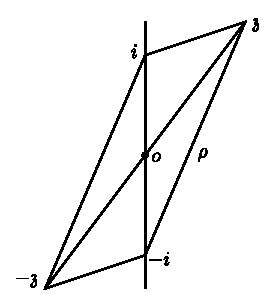
\includegraphics{vol2-figures/fig2.34.eps}}
  \end{figure}
\end{minipage}
\medskip

Actually we take only $\rho, \sigma > 0$; we shall exclude the points
$i$ and $z$ themselves. Then this becomes
$$
- \frac{1}{4 i} \frac{e^{\pi N (\rho i + \sigma \mathfrak{z})}+ e^{-
    \pi N (\rho i + \sigma \mathfrak{z})}}{e^{ \pi N(\rho i + \sigma
    \mathfrak{z})}- e^{- \pi N (\rho i + \sigma \mathfrak{z})}} \times
i \times \frac{e^{ \pi i N (\rho i + \sigma
    \mathfrak{z})/\mathfrak{z}} + e^{- \pi i N ( \rho i + \sigma
    \mathfrak{z})/\mathfrak{z}}}{e^{\pi i N (\rho i + \sigma
    \mathfrak{z})/\mathfrak{z}}- e^{- \pi i N (\rho i + \sigma
    \mathfrak{z})/\mathfrak{z}}} 
$$

The size of the first factor is determined by the terms $e^{\pi N
  \sigma \mathfrak{z}}$ and $e^{- N \pi \sigma \mathfrak{z}}$ in the
numerator; the first term becomes big and the other goes to zero as $N
\to \infty (\sigma > 0~\text{and}~ \mathcal{R}_e \mathfrak{z}> 0)$. So
we divide by the first term. Similarly for the second factor. We
therefore get
$$
- \frac{1}{4} \frac{1+ e^{-2 \pi N (\rho i + \sigma \mathfrak{z})}}{1-
  e^{-2 \pi N (\rho i + \sigma \mathfrak{z})}} \cdot \frac{e^{- 2 \pi
    N \left(\frac{\rho}{\mathfrak{z}} + \frac{\sigma}{i}
    \right)}+ 1}{e^{- 2 \pi N \left( \frac{\rho}{\mathfrak{z}} +
    \frac{\sigma}{i}\right)}-1} 
$$\pageoriginale

As $N \to \infty$ the exponential factors go to zero; so the whole
expression tends to $\frac{1}{4}$. It will further remain on its way
bounded, because the numerators in either factor are at most equal to
2, while the denominators remain away from zero by a fixed amount, as
we shall be showing in a moment - and for this it is essential to have
$N= n+ \frac{1}{2}$. 

Since the functions concerned are even functions, what was good here
would also be good on the apposite side, from $x=- i$ to $x=-z$. So on
this side also the expression will tend to $\frac{1}{4}$. We cannot
say uniformly; indeed if $\sigma=0$, here is no convergence in the
first factor, and if $\rho =0$ none in the second factor, though there
is boundedness: the thing would oscillate finitely.

Now take the other pieces of $x F_n (x)$ on the same sides of
$\rho$. We have to consider
$$
\frac{e^{2 \pi \mu \frac{N}{k} (\rho i + \sigma \mathfrak{z})}}{1-
  e^{2 \pi N (\rho i + \sigma \mathfrak{z})}} \times \frac{e^{- 2 \pi
    i \mu^* \frac{N}{k \mathfrak{z}} (\rho i +\sigma
    \mathfrak{z})}}{1- e^{-2 \pi i \frac{N}{\mathfrak{z}} (\rho i +
    \sigma \mathfrak{z})}}
$$

Remember, what is now important, that $0< \mu < k$, but neither 0 nor
$k$. The denominator in the first factors goes more strongly to
infinity as $N \to \infty$ than the numerator because $\frac{\mu}{k}$
is a proper fraction; so too in the second factor because $\mu >
1$. So the whole function tends to zero. Hence on these two sides $x
F_n (x) \to \frac{1}{4}$. 

Now\pageoriginale consider the other two sides; it looks different
here and has got to be inspected. On the side from $x= -i$ to $x= z$,
$x= - \rho i + \sigma \mathfrak{z}$; $\sigma, \rho > 0$, $\sigma+ \rho
=1$, and the first part of $xF_n(x)$ is 
\begin{align*}
  - \frac{1}{4i} \cot h \pi N x \cot \frac{\pi N x}{\mathfrak{z}} & =
  - \frac{1}{4} \frac{e^{ \pi N (- \rho i + \sigma \mathfrak{z})} +
  - e^{- \pi N( - \rho i + \sigma \mathfrak{z})}}{e^{\pi N(- \rho i +
  - \sigma \mathfrak{z})}- e^{- \pi N (- \rho i + \sigma
  - \mathfrak{z})}}\\
  & \hspace{3cm}\times \frac{e^{ \pi i N \left( \frac{-\rho i}{\mathfrak{z}} +
   \sigma\right)} + e^{- \pi i N \left( \frac{-\rho i}{\mathfrak{z}} +
  - \sigma\right)}}{e^{\pi i N \left( \frac{-\rho}{\mathfrak{z}} i +
   \sigma \right)} - e^{- \pi i N \left( -\frac{\rho i}{\mathfrak{z}}
   + \sigma\right)}}\\
  & = - \frac{1}{4} \frac{1+ e^{- 2 \pi N (-\rho i + \sigma
  \mathfrak{z})}}{1- e^{- 2 \pi N (- \rho i + \sigma \mathfrak{z})}}
  - \times \frac{1+ e^{-2 \pi i N \left( - \frac{\rho i}{\mathfrak{z}}
  + \sigma \right)}}{1- e^{- 2 \pi i N \left(- \frac{\rho
  - i}{\mathfrak{z}} + \sigma \right)}}
\end{align*}

Let $N \to \infty$. Assuming that the denominator is going to behave
decently, this goes to $- \frac{1}{4}$. The other pieces go to zero
for the same reason as before. And all this is good for the opposite
side too.

We now have got to show that the convergence it nice and the
denominators do not make any fuse. This we can clarify in the
following way. Consider the denominator $1- e^{- 2 \pi N (\rho i +
  \sigma \mathfrak{z})}$. 

Difficulties will arise if the exponent comes close to an even
multiple of $\pi i$. So we should see that it stays safely away from
these points. 

\begin{figure}[H]
  \centering{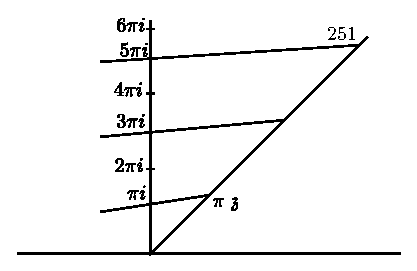
\includegraphics{vol2-figures/fig2.35.eps}}
\end{figure}

And\pageoriginale actually it stays away from the danger spots by the same distance,
for the exponent is $- 2N (\pi i \rho + \pi \mathfrak{z} \sigma)$
i.e., a point on the segment joining $( 2r+1)\pi i$ and $(2 r +1) \pi
\mathfrak{z}$. Since $e^{\mathfrak{z}}$ is periodic there is a minimal
amount by which it stays away from 1. The second denominator looks a
little different. We have $\frac{\pi}{\mathfrak{z}}$ instead of $\pi
\mathfrak{z}$. But we have only to turn the whole thing around. We see
how essential it was to take $N= n + \frac{1}{2} = (2n+1)\frac{1}{2}=
$ on odd multiple of $\frac{1}{2}$. 

So the convergence is nice, but not uniform. We can nevertheless say
that $xF_n (x) \to \pm \frac{1}{4}$ boundedly on the sides of $\rho$
except for the vertices where it does not converge but oscillates
finitely. But bounded convergence is enough for interchanging
integration and summation. $F_n (x) \to \pm \frac{1}{4x}$ and the $x$
does not ruin anything because it stays away from zero everywhere on
$\rho$. Hence
$$
\lim\limits_{n \to \infty} \frac{1}{2 \pi i} \int_p F_n (x) dx
$$
exists and we have
\begin{align*}
  \lim\limits_{n \to \infty} \frac{1}{2 \pi i} \int_p F_n (x) dx & =
  \frac{1}{2 \pi i} \int_p \pm \frac{1}{4x} dx\\
  & = \frac{1}{2 \pi i} \left\{ \int\limits_{\mathfrak{z}}^i \frac{dx}{4x} -
  \int^{-\mathfrak{z}}_{i} \frac{dx}{4x} + \int^{-i}_{-\mathfrak{z}}
  \frac{dx}{4x} - \int^{\mathfrak{z}}_{-i} \frac{dx}{4x} \right\}\\
  & = \frac{1}{8 \pi i} \left\{ \int^i_{\mathfrak{z}} \frac{dx}{x} -
  \int^{\mathfrak{z}}_{-i} \frac{dx}{x} + \int^i_{\mathfrak{z}}
  \frac{dx}{x} - \int^{\mathfrak{z}}_{-i} \frac{dx}{x}\right\}\\
  & = \frac{1}{4 \pi i} \left\{ \int^i_{\mathfrak{z}} \frac{dx}{x} -
  \int^{\mathfrak{z}}_i  \frac{dx}{x}\right\}
\end{align*}
$z$\pageoriginale is in the positive half-plane; we can take the principal branch of
  the logarithm, so that we get on integration, since $\log i$ is
  completely determined,
$$
    \frac{1}{4 \pi i}  \left\{  \frac{\pi}{2} - \log \mathfrak{z} - \left(
    \log \mathfrak{z} + \frac{\pi i}{2}\right)\right\} 
     = - \frac{1}{2 \pi i} \log \mathfrak{z}
$$

    \begin{figure}[H]
      \centering{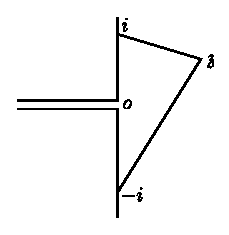
\includegraphics{vol2-figures/fig2.36.eps}}
    \end{figure}


So we have proved the foreseen formula with the particular
substitution $C (h, k)= s(h, k)- \frac{h-h'}{12k}$:
$$
\log \eta \left( \frac{h'+ i/\mathfrak{z}}{k}\right) = \log \eta
\left(\frac{h + i \mathfrak{z}}{k} \right)+ \frac{1}{2} \log
\mathfrak{z} + \pi i s(h, k) + \pi i \frac{h'-h}{12k},
$$
which\pageoriginale is the complete formula in all its details. The
mysterious $s(h, k)$ enjoys certain properties. It has the group
properties of the modular group behind it and so must participate in
them. 


